\documentclass[a4paper,norsk]{article}
\usepackage[latin1]{inputenc}
\usepackage[T1]{fontenc}
\usepackage{babel,textcomp,listings, subfigure,graphicx}
                                    
\title{Triangle Cavity Flow}
\author{Sebastian Gjertsen}
\begin{document}
\maketitle
\begin{center}
\section*{Introduction}
In this study I have looked at steady 2-D incompressible flow inside a cavity driven triangle. This seemingly simple geometry gives interesting flows for different Reynolds number, and the implementation is rather easy to check with published papers. I used [Erturk and Gokcol] and [Spectral element book]  as a reference to make mesh and to look at formation of eddies. The goal will be to compare results with [Erturk and Gokcol] and [Spectral element book] , and discuss results.
\end{center}
\section*{Numerics}
I used the FEniCS software with Oasis, which solves the Navier-Stokes equations both transient and steady. 


\section*{Results)}
First I considered an equilateral Triangle with corner points: \newline
a = (-$\sqrt(3)$, 1), b = ($\sqrt(3)$, 1) ,c = (0, -2) \newline
\begin{figure}
    \centering
    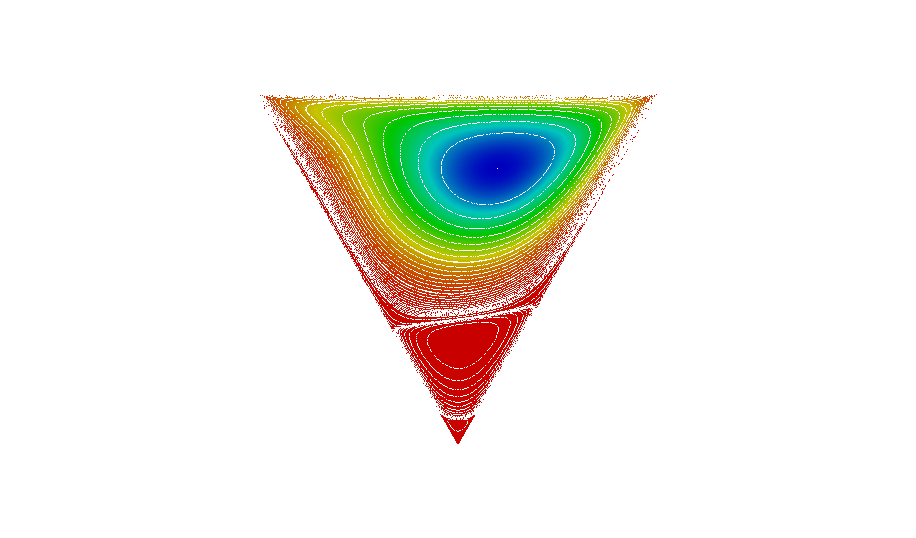
\includegraphics[trim = 25mm 0mm 25mm 0mm, clip, scale=0.4]{Equilateral_Re_100.png}
    \caption{Streamfunction of equilateral triangle}
    \label{fig:awesome_image}
\end{figure}
\newline
Where the Reynolds number is defined as $Re = \frac{U}{\mu} $, where i set $U=1$ and controlled Re by changing $\mu$
\newline
The table looks at the position of the center eddy and the value of the streamfunction and vorticity at this point. \newline
This study was done with 73541 vertices and 145664 cells
\newline
\begin{tabular}{l*{6}{c}r}
   & &Erturk and Gockol & & & Me\\
   \hline 
  Re & $\psi$ & $\omega$ &(x,y) & $\psi$ & $\omega$ & (x,y)  \\
  1   &   -0.2329  &-1.3788  & (0.0101, 04668) &-0.2329 & -1.3658  & (0.0109, 0.4617)  \\
  50   &  -0.2369 & -1.4689 & (0.3484, 04434)  & -0.2367 &-1.4708 & (0.3525, 0.4467)    \\
  100  & -0.2482 & -1.3669 & (0.3315, 0.3555)   & -0.2476 & -1.3599 &(0.3339, 0.3576)  \\
  200   & -0.2624 &-1.2518  & (0.2030, 0.2734)  & -0.2613 & -1.2459 & (0.1978, 0.2758 ) \\
  350   & -0.2724 & -1.1985 & (0.1556, 0.2383) &-0.2708 & -1.1887 & (0.1605, 0.2412)   \\
  500   & -0.2774 & -1.1791 &  (0.1319, 0.2207)  & -0.2754 &  -1.1666 & (0.1395, 0.2237)       \\
  750   &  -0.2818 & -1.1668 &  (0.1150, 0.2031) & -0.2793  & -1.1504  & (0.1160, 0.2056 ) \\
  1000   & -0.2844 & -1.1629 &(0.1116, 0.1973) & -0.2814  & -1.1427 & (0.1066, 0.1944) \\
  1250   & -0.2861 & -1.1624 & (0.1049, 0.1973) & -0.2826 & -1.1382 & (0.1066, 0.1944)   \\
  1500   & -0.2872 & -1.1639 & (0.1015, 0.1914)  & -0.2834 & -1.1354  & (0.1022, 0.1828)\\
  1750   &  -0.2881 & -1.1675 & (0.1015, 0.1914) &   &\\ 
\hline
\end{tabular}
\newline
\newline
\newline 
Next I considered an Isoceles Triangle with corner points: \newline
a = (-1, 0), b = (1, 0) ,c = (0, -4), with 64051 vertices and 126444 cells\newline
\newline

\begin{figure}
    \centering
    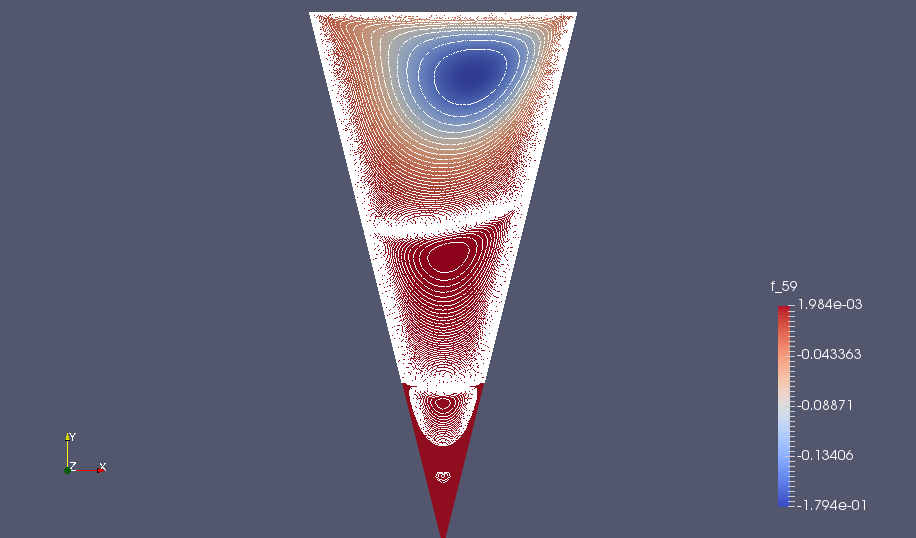
\includegraphics[trim = 100mm 0mm 100mm 0mm, clip, scale=0.4]{isoceles_Re_100.png}
    \caption{Streamfunction of isoceles triangle}
    \label{fig:awesome_image}
\end{figure}
In this table we also looked at the position and value of the center-eddy:
\newline
\begin{tabular}{l*{6}{c}r}
   & Erturk and Gockol & Me\\
   \hline 
  Re &(x,y) & (x,y)  \\
12.5 & (0.059, -0.391) & (0.0587, -0.4001 )\\
25 & (0.115,-0.398) &  (0.1101, -0.3999 )\\
100 & (0.213, -0.477)& (0.2124, -0.4767 ) \\
200 & (0.129, -0.563)& (0.1275, -0.5608 )\\  
\hline
\end{tabular}
\newline
\newline
The next thing i looked at was where the second eddy was. This eddy is spinning the opposite direction so i had to look for the highest value of the stream function:
\newline
\begin{tabular}{l*{6}{c}r}
   & Me\\
   \hline 
  Re & $\psi$ & $\omega$& (x,y)   \\
12.5 & 0.0002 & 0.0108 & (-0.0018, -2.1924)\\
100 & 0.0020 & 0.0699  & (0.0490, -1.8199)\\
200 &  0.0073 & 0.2183 & (-0.0237, -1.6809)\\
\hline
\end{tabular}
\newline
\newline
The next thing i looked at was how many eddies i could find. According to [Spectral] every eddy formed will be 406 times weaker then the previous. So the velocities and the very bottom eddies will be very small. To find these eddies I looked at the absolute velocities in the horizontal direction on a line straight through the mesh from the top at (0.0) to (0,-4). As we can see when the plot has a dip is where the velocities have changed direction and where we can find the eddies center. I used a very fine mesh at the bottom to catch as many eddies as a could. After a careful count, i got 9 eddies. This was done with Re=1, and with a mesh consisting of 57843 vertices and 113176 cells.\newline
We can see that near the bottom we get disturbances when the eddies becomes to small for the mesh. One could argue that with a fine enough mesh the number of eddies would go to infinity.

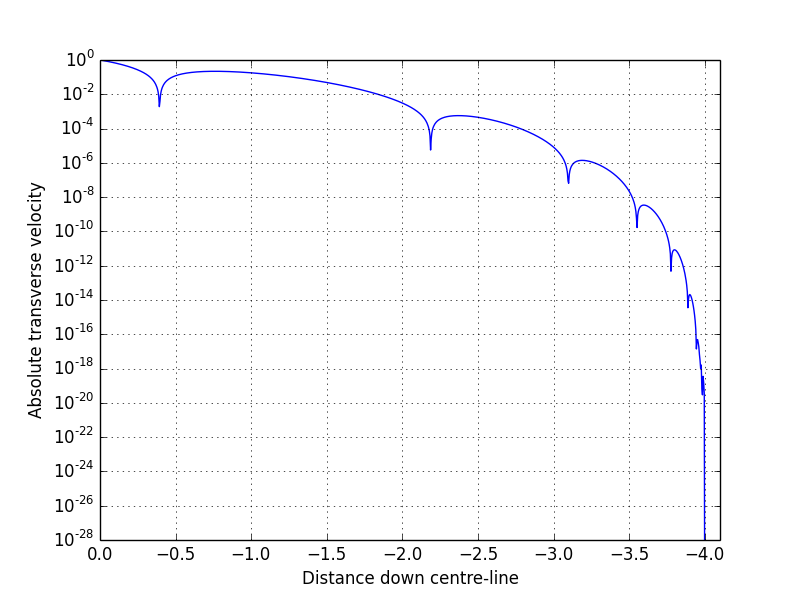
\includegraphics[trim = 0mm 0mm 0mm 0mm, clip, scale=0.4]{eddy_plot_1.png}
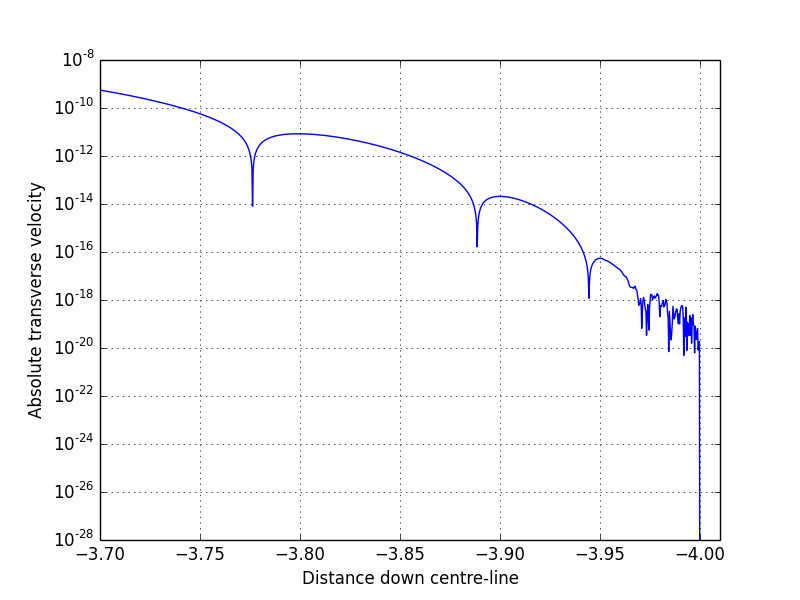
\includegraphics[trim = 0mm 0mm 0mm 0mm, clip, scale=0.4]{eddy_plot_2.png}









\end{document}